A \emph{scalar field}\index{scalar field}
is a function that assigns each point in space a
scalar value.  For example, given latitude and longitude $(x,y)$,
the function that outputs the elevation of the surface of the earth
at position $(x,y)$ is a scalar field.  However,
we might ask for a function that when given $(x,y)$ returns
a vector (maybe the velocity of the wind at that point on the earth).
Functions that assign a vector to each point in space
are called \emph{vector fields}\index{vector field}.

Vector fields are key in physics because they model
vector quantities that are non-constant with respect to
space.  For example, force is a vector!  The force due to of gravity
around a point mass is always directed towards the origin---that
means, as you move in space, the direction of the force 
changes.  Suppose there is a point mass at the origin.
We might model the force\footnote{ Despite what is peddled in
Star Wars, this is a real \emph{force field}.} due to this point mass acting on a particle
at position $(x,y,z)$ with the vector field
\[
	\vec F(x,y,z) = \tfrac{1}{(x^2+y^2+z^2)^{3/2}}\mat{-x\\-y\\-z}.
\]
Indeed, the vector $\vec F(x,y,z)$ always points towards the origin,
and $\norm{\vec F(x,y,z)}=\frac{1}{x^2+y^2+z^2}$ is $1/d^2$ where $d$
is the distance from the origin.


\subsection{Notation}
Notationally, $\vec F:\R^n\to\R^m$ indicates that $\vec F$ inputs points or vectors in $\R^n$
and outputs points or vectors in $\R^m$.  Oftentimes in physics $n=m$, but doesn't need to.

When defining a vector field, sometimes it's convenient to use components
and sometimes it's easier to work with vectors.  For example, the force field
$\vec F:\R^2\to\R^3$ above was defined in terms of components as
\[
	\vec F(x,y,z) = \tfrac{1}{(x^2+y^2+z^2)^{3/2}}\mat{-x\\-y\\-z},
\]
but we could have equivalently defined it using vectors by the equation
\[
	\vec F(\vec v) = -\frac{\vec v}{\norm{\vec v}^3}.
\]


\section{Graphing Vector Fields}

Traditionally, a function $f:\R\to\R$ is graphed on a coordinate
plane by picking one axis to be the domain, one
axis to be the range, and then putting a point at each pair $(x,f(x))$.
For a function $g:\R^2\to\R$, we do something similar, except, this time,
the domain is a plane.  But, no matter, we arrange a third axis orthogonal
to a plane and graph points $(x,y,f(x,y))$ in this three-dimensional space.

With vector fields, we cannot graph in the same way.  A vector field
$\vec F:\R^2\to\R^2$ inputs vectors in a plane and outputs vectors in
a plane. To traditionally ``graph'' this function, we would need to
plot points in $\R^2\times\R^2=\R^4$.  Four-dimensional plots are hard to make!
Fortunately, the goal of graphing is rarely to make a faithful representation
of a function---it is to make a visual representation of a function
to aid our thinking.  With this perspective, representing four-dimensional
graphs won't be hard.

If we think of $\vec F:\R^2\to\R^2$ as attaching a vector to each point in
$\R^2$, we might graph $\vec F$ by drawing vectors at each point in $\R^2$.

XXX Figure

This type of plot is called a \emph{quiver plot}\index{quiver plot},
and it will be the main way we visualize vector fields.

\begin{example}
	Graph the vector field $\vec F:\R^2\to\R^2$ defined by $\vec F(x,y)=\mat{x\\y}$.

	XXX Finish
\end{example}

When making a quiver plot, there are two things to consider: (i) how
densely do you draw vectors, and (ii) how do you scale the vectors?
The answer to these two questions depends on the situation---remember,
the goal of plotting a vector field is to visualize what is happening.

Consider the vector field $\vec A:\R^2\to\R^2$ defined by $\vec A(x,y)=\mat{-y\\x}$.
If we plot vectors every $0.5$ units and plot the vectors at the same scale
as the domain, we get the following, hard to follow, figure.

XXX Figure

However, if we plot vectors every $0.5$ units but scale the vectors so they are
$1/4$ the size they'd conventionally be, we get a much more understandable figure.

XXX Figure

We might even decide that the magnitude of each vector is not so important
and totally ignore it in our plot.

XXX Figure with unit vectors


\begin{exercises}
\end{exercises}

\section{The Gradient}

We already have familiarity with one class of vector fields---gradients.
Given a differentiable function $f:\R^n\to\R$, we can always consider the
vector field $\nabla f:\R^n\to\R^n$.  And, $\nabla f$ has some nice geometric
properties.  For instance, $\nabla f$ always points in the direction
of greatest change for $f$.

XXX Figure surface with vector field at base

The connections between $f$ and $\nabla f$ run deep.  Suppose
for a moment that $f:\R^2\to\R$ is affine.  That is, $f(x,y)=\alpha x+\beta y+\gamma$. 
Now, $\nabla f(x,y)=\mat{\alpha\\\beta}$ is
constant.  If $\vec a,\vec b\in\R^2$, we can consider the change in height
of $f$ when moving from $\vec a$ to $\vec b$.  This is,
\[
	f(\vec b)-f(\vec a) = \alpha b_x+\beta b_y - \alpha a_x - \beta a_y
	=\nabla f(\vec a)\cdot (\vec b-\vec a).
\]
Of course this is no surprise---we first encountered
gradients when finding affine approximations of
functions.  Baked into the very core of the gradient is the fact that for a 
differentiable function $h:\R^n\to\R$,
\[
	h(\vec b)-h(\vec a)=\text{change in }h\text{ from }\vec a\text{ to }\vec b
	\approx \nabla h(\vec a)\cdot (\vec b-\vec a),
\]
so long as $\vec a$ and $\vec b$ are close together.  Now, let's apply
some calculus reasoning.

Let $h:\R^n\to\R$ be a differentiable function and let $\vec a,\vec b\in\R^n$
be points that \emph{aren't} close to each other.  Let $\vec a=\vec x_1,\vec x_2,\ldots,\vec
x_m=\vec b$ be a sequence of points so that $\norm{\vec x_{k+1}-\vec x_k}$ is small.
We may think of $\vec x_i$ as a sequence of tiny steps used to get from $\vec a$ to
$\vec b$.  Now, we have
\[
	h(\vec b)-h(\vec a)=\text{change in }h\text{ from }\vec a\text{ to }\vec b
	\approx 
	\sum \nabla h(\vec x_k)\cdot (\vec x_{k+1}-\vec x_k).
\]
If we define $\Delta \vec x_k=\vec x_{k+1}-\vec x_k$, we get an eerily familiar
formula:
\[
	h(\vec b)-h(\vec a)
	\approx 
	\sum \nabla h(\vec x_k)\cdot \Delta \vec x_k.
\]
On the left we have the scalar quantity $h(\vec b)-h(\vec a)$ and on the right
we have a Riemann sum approximation of the vector line integral\index{vector line integral}
of $\nabla h$ along some path starting at $\vec a$ and ending at $\vec b$.  After
taking a limit, this approximation becomes exact.

\begin{theorem}
	\label{THMFTC1}
	Let $h:\R^n\to\R$ be a differentiable function and let
	$\mathcal C\subset \R^n$ be a parameterized, bounded curve 
	which starts at $\vec a\in\R^n$ and ends at $\vec b\in\R^n$.
	Then,
	\[
		h(\vec b)-h(\vec a) = \int_{\mathcal C} \nabla h\cdot \d\vec r,
	\]
	where $\int_{\mathcal C} \nabla h\cdot \d\vec r$ is the vector line
	integral of $\nabla h$ along $\mathcal C$.
\end{theorem}

Theorem \ref{THMFTC1} should remind you of the fundamental theorem of calculus,
which states for a differentiable function $f:\R\to\R$, 
\[
	f(b)-f(a) = \int_a^b f'.
\]
In one dimension, there aren't many ways to get between two points.  In
contrast, there are infinitely many ways to get between two points
in higher dimensions.  Theorem \ref{THMFTC1} says that all these ways
are equivalent, and that $\nabla h$ takes the place of $h'$.

\subsection{Orientation}

As we delve into the realm of vector fields, we need to take note of something
new---orientation\index{orientation}.  In a scalar line integral of $f$ along the curve
$\mathcal C$, we added up the ``height'' of $f$ along the curve $\mathcal C$.
It didn't matter how we traverse $\mathcal C$, and so it
doesn't matter how we parameterize $\mathcal C$ when computing $\int_C f$.  
The area of the graph of $f$ above
$\mathcal C$ depends only on $f$ and $\mathcal C$.  However, things are different for
vector line integrals.

If $\mathcal C$ connects the points $\vec a$ and $\vec b$ and we wish to compute
the amount of work done by the force field $\vec h$ when moving from $\vec a$ to
$\vec b$ along $\mathcal C$, not all parameterizations of $\mathcal C$ will
do.  We must parameterize $\mathcal C$ such that we start at $\vec a$ and
end at $\vec b$.  Thus, the vector integral $\int_{\mathcal C} \vec h\cdot \d\vec r$
depends not only on $\vec h$ and $\mathcal C$, but also on the direction
or \emph{orientation}\index{oriented curve} of $\mathcal C$.

For curves, there are only two orientations, forwards and backwards,
and reversing the orientation of a curve in a vector line integral just multiplies
the result by $-1$.

\begin{example}
	XXX simple example with orientation flipped
\end{example}


The concept of orientation is familiar from single-variable calculus.
After all,
\[
	\int_a^b f=-\int_b^a f.
\]

From now on, if it matters, we will always specify a curve with
its orientation.  If the curve is closed, we will specify its orientation
as \emph{clockwise} or \emph{counterclockwise}.

\subsection{Conservative Vector Fields}

Theorem \ref{THMFTC1} shows that gradients and vector line integrals
interact nicely.  So nicely, in fact, that vector fields coming 
from gradients have a special name.

\begin{definition}[Conservative Vector Field \& Potential Function]
	A vector field $\vec h:\R^n\to\R^n$ is called \emph{conservative}
	if there is some function $f:\R^n\to\R$ so that $\nabla f=\vec h$.
	Such an $f$ is called a \emph{potential function for $\vec h$}.
\end{definition}

We can think of conservative vector fields\index{conservative vector field}
as those having anti-derivatives,
called \emph{potential functions}\index{potential function}\footnote{
In math, if $\nabla f=\vec h$, we say $f$ is a potential function for $\vec h$.
In physics you say that $-f$ is a potential function for $\vec h$---this aligns
more closely with a physicist's notion of \emph{potential energy}.}.  Once
we have a potential function $f$ for a vector field $\vec h$, 
Theorem \ref{THMFTC1} shows that we can compute vector line integrals
of $\vec h$ by evaluating $f$ on the endpoints of our path.  An immediate consequence
is that the integral around a closed path in a conservative vector field is
zero.

\begin{example}
	XXX Example --- work on a hill via complicated path and sub for
	and easy path.
\end{example}

Since conservative vector fields make vector line integrals so easy, it's useful
to determine whether a given vector field is conservative.  The only sure-fire
way to determine a vector field is conservative is to find a potential function.
However, there are several heuristics for showing that a vector field is not
conservative.

\bigskip

Having established that conservative vector fields are useful,
it would be nice to be able to decide if a given vector field is
conservative.  The only sure-fire way to do so is to produce a 
potential function.  However, there methods we can use to quickly
determine if a particular vector field \emph{cannot} be conservative.

The \emph{screening test}\index{screening test} 
\label{SECSCREENING}
is one such method.  Suppose that $\vec F=\mat{F_x\\F_y}$
and that $\vec F$ is conservative.  That means $\vec F=\nabla f$
for some potential function $f:\R^2\to\R$, and so
\[
	F_x = \frac{\partial f}{\partial x}\qquad\text{and}\qquad 
	F_y=\frac{\partial f}{\partial y}.
\]

If $\vec F$ is a \emph{nice} vector field (that is, it comes from a sufficiently differentiable
$f$), then
\[
	\frac{\partial F_x}{\partial y} = 
	\frac{\partial^2 f}{\partial y\partial x} = 
	\frac{\partial^2 f}{\partial x\partial y} = 
	\frac{\partial F_y}{\partial x}. 
\]

This means that if $\frac{\partial F_x}{\partial y} \neq \frac{\partial F_y}{\partial x}$,
we can conclude that $\vec F$ is \emph{not} conservative.

\begin{example}
	Is the vector field $\vec F(x,y)=\mat{x+1\\y+x^2}$ conservative?

	Define $F_x(x,y)=x+1$ and $F_y(x,y)=y+x^2$ so that $\vec F  =\mat{F_x\\F_y}$.
	Now,
	\[
		\frac{\partial F_x}{\partial y} = 0
		\neq 2x = 
		\frac{\partial F_y}{\partial x},
	\]
	and so $\vec F$ is not conservative.
\end{example}

It should be noted that the screening test can only prove vector fields
are not conservative.  It cannot be used to show that they are!

\begin{example}
	Is the vector field
	$\vec F(x,y) = \mat{\frac{-y}{x^2+y^2}\\[4pt]\frac{x}{x^2+y^2}}$ conservative?

	Defining $F_x(x,y)=\frac{-y}{x^2+y^2}$ and $F_y(x,y)=\frac{x}{x^2+y^2}$
	so that $\vec F = \mat{F_x,F_y}$, we compute
	\[
		\frac{\partial F_x}{\partial y} = \frac{y^2-x^2}{(x^2+y^2)^2}
		= 
		\frac{\partial F_y}{\partial x},
	\]
	and so the screening test cannot be used to conclude anything
	about whether or not $\vec F$ is conservative.

	
	However, letting $\mathcal C$ be the circle of radius 1 centered at the
	origin and oriented counter clockwise, we compute $\int_{\mathcal C} \vec F\cdot \d \vec r
	=2\pi$.  If $\vec F$ were a conservative vector field, the 
	vector line integral around any closed path would be $0$.  Thus, we conclude
	that $\vec F$ is not conservative.
	
\end{example}

The screening test works analogously for higher-dimensional vector fields.  One just
needs to test all combinations of mixed partials---if any combination fails, the vector
field is not conservative.

\begin{exercises}
\end{exercises}


\section{Flux and Divergence}

Suppose that the vector field $\vec F(x,y,z)=(4,0,0)$
describes the velocity of water in a river of uniform density.
You cast a $1\times 1$ square net in the river with normal
vector $(1,0,0)$ and ask the following question: how much 
water per unit time is flowing through the net?

XXX Figure

In this situation, it is easy to compute.  Let us assume
the density of the water is $1$.  In this case, since the direction
of flow is orthogonal to the net (because the normal vector is parallel
to the direction of flow), we know
\[
	\text{mass}/\text{unit time} = (\text{net area})
	(\text{water speed})=(1)(4)=4.
\]

If we angle the net slightly, so that it has a normal vector
$(1,1,0)$, computing the amount of water that goes through
the net in a time unit is still not so bad.
\[
	\text{mass}/\text{unit time} = (\text{perceived net area})
	(\text{water speed}).
\]
Here, the \emph{perceived net area} is the area that the net appears to
the water.  Since the net is angled at $45^\circ$ relative to the flow
of the water, the net \emph{appears} smaller, from the perspective of the water.

XXX Figure showing ``apparent'' height

To the water, the net appears to have width $1$ and height $\sqrt{2}/2$, giving
the net a perceived area of $\sqrt{2}/2$.  Now we can compute
\[
	\text{mass}/\text{unit time} = (\text{perceived net area})
	(\text{water speed}) =\tfrac{\sqrt 2}{2}(4)=2\sqrt{2}.
\]

Equivalently, we could have thought about water from the perspective of the net.
We know
\[
	\text{mass}/\text{unit time} = (\text{net area})
	(\text{water speed normal to net}),
\]
and computing the velocity of water normal to the net can be done with a dot product.
In particular,
\[
	\text{water speed normal to net}=\Proj_{\vec n}\vec v = \mat{2\\2\\0},
\]
where $\vec n=(1,1,0)$ is the normal vector for the net and $\vec v=(4,0,0)$
is the velocity vector of the water.  Now
\begin{align*}
	\text{mass}/\text{unit time} &= (\text{net area})
	(\text{water speed normal to net}) \\
	&= (1)\norm*{\mat{2\\2\\0}}=2\sqrt{2},
\end{align*}
which is the same quantity we computed before.

Measuring how much a vector field ``flows'' through a surface $\mathcal S$
is called the \emph{flux}\index{flux}\footnote{
The term \emph{flux} comes from \emph{fluxus},
which means ``flow'' in Latin.
} of the vector field through $\mathcal S$, and comes up in applications
ranging from fluid mechanics to electro-magnetism and relativity gravity.

\subsection{Computing Flux}

Given constant vector fields and flat surfaces, flux is not difficult to compute.
However, the vector fields we encounter in nature are rarely constant and
the surfaces are rarely flat.  But, the ideas of calculus are here
to help us!

By now, we are familiar with the idea of chopping things up into little pieces,
approximating each piece, adding them together again, and taking a limit.  Finding
the flux of a vector field through an arbitrary surface follows this pattern.

Let $\vec F:\R^3\to\R^3$ be a smooth vector field and let $\mathcal S$ be 
a surface\footnote{ An orientable surface, to be precise.}.
Let $\Delta A$ represent a tiny patch of the surface $\mathcal S$.  We can then say
\[
	\Flux_{\mathcal S} \vec F = \sum_{\Delta A} \Flux_{\Delta A} \vec F,
\]
where $\Flux_A \vec B$ means the flux of the vector field $\vec B$ through the
surface $A$.  This looks a lot like a setup for a surface integral!  Let's make
the connection exact.

Let $\vec p:\R^2\to\mathcal S$ be a parameterization of the surface $\mathcal S$,
and let $\Delta A_{(x_0,y_0)}=\vec p([x_0,x_0+\Delta x]\times [y_0,y_0+\Delta y])$
be a tiny sector of $\mathcal S$ with ``lower-left corner'' at $\vec p(x_0,y_0)$.
As long as $\Delta x$ and $\Delta y$ are small, $\Delta A_{(x_0,y_0)}$ will be
small.

Now, let's approximate.  Since $\Delta A_{(x_0,y_0)}$
is small, we could approximate $\vec F$ near $\Delta A_{(x_0,y_0)}$
by the constant vector 
field $\vec F_{(x_0,y_0)}(x,y) = \vec F\circ \vec p(x_0,y_0)$.  Further,
if $\Delta x$ and $\Delta y$ are small enough, we can approximate $\Delta A_{(x_0,y_0)}$
by a tiny parallelogram coming from the 
canonical parameterization of the tangent plane to $\mathcal S$ at $\vec p(x_0,y_0)$.

Recall, given the parameterization $\vec p$,
the canonical parameterization of the tangent plane to $\mathcal S$ at $\vec p(x_0,y_0)$
is
\[
	\vec P(t,s) = t \frac{\partial \vec p}{\partial x}(x_0,y_0) + 
	s\frac{\partial \vec p}{\partial y}(x_0,y_0)
	+\vec p(x_0,y_0).
\]
Since $\vec P$ is a canonical parameterization, if $\Delta x$ and $\Delta y$
are small, then 
\[
\Delta A_{(x_0,y_0)}=\vec p([x_0,x_0+\Delta x]\times [y_0,y_0+\Delta y])
\approx \vec P([x_0,x_0+\Delta x]\times [y_0,y_0+\Delta y]).
\]
Further, $\vec P([x_0,x_0+\Delta x]\times [y_0,y_0+\Delta y])$ is a parallelogram
with normal vector
\[
	\vec n = \frac{\partial \vec p}{\partial x}(x_0,y_0) \times
	\frac{\partial \vec p}{\partial y}(x_0,y_0)
\]
and area $\norm{\vec n}\Delta x\Delta y$.

We have developed several approximations.  Before we put them all together, let's
give them simple names.  Fix $x_0$ and $y_0$,
and let $\Delta A=\Delta A_{x_0,y_0}$;
let $Q(x,y) = \vec F\circ \vec p(x_0,y_0)$ be a constant
vector field approximating $\vec F$; and, let 
$\Delta R=\vec P([x_0,x_0+\Delta x]\times [y_0,y_0+\Delta y])$ be a parallelogram
approximating $\Delta A$.  We then have, so long as $\Delta x$ and $\Delta y$ are small
\begin{align*}
	\Delta A &\approx \Delta R\\
	\vec F &\approx \vec Q.
\end{align*}
Putting this all together, 
\begin{align*}
	\Flux_{\Delta A}\vec F
	\approx \Flux_{\Delta A}\vec Q 
	\approx \Flux_{\Delta R}\vec Q
\end{align*}

Now, $\tfrac{\vec n}{\norm{\vec n}}$ is a unit normal vector to $\Delta R$,
and so
\[
	\Flux_{\Delta R}\vec Q = 
	\underbrace{\norm{\vec n}\Delta x\Delta y}_{\text{area of $\Delta R$}}\tfrac{\vec n}{\norm{\vec n}}\cdot \vec Q
	=\vec n\cdot \vec Q\Delta x\Delta y.
\]
Substituting in for $\vec n$ and $\vec Q$, we have
\begin{equation}
	\label{EQFLUXAPPROX}
	\Flux_{\Delta A}\vec F
	\approx 
	\left(\frac{\partial \vec p}{\partial x}(x_0,y_0) \times
	\frac{\partial \vec p}{\partial y}(x_0,y_0)\right)
	\cdot \Big(\vec F\circ \vec p(x_0,y_0)\Big )\Delta x \Delta y.
\end{equation}

We worked pretty hard to get Equation \eqref{EQFLUXAPPROX}, but
let's remind ourselves that the idea was simple.  We approximated
a changing vector field by a constant one and a curvy shape by a flat one.
The rest of the formula comes from exploiting the relationship between
the cross product and the area of a parallelogram and the computation
of the flux of a constant vector field through a flat surface.

Finally, since 
\[
	\Flux_{\mathcal S} \vec F = \sum_{\Delta A} \Flux_{\Delta A} \vec F
\]
and we have approximated $\Flux_{\Delta A}\vec F$, we may take a limit to obtain
\begin{align*}
	\Flux_{\mathcal S} \vec F &= \sum_{\Delta A} \Flux_{\Delta A} \vec F\\
	&=\lim_{\Delta x,\Delta y\to 0} \sum_{\Delta R} \Flux_{\Delta R} \vec F\\
	&= \int_{\mathcal S} 
	\left(\frac{\partial \vec p}{\partial x}(x,y) \times
	\frac{\partial \vec p}{\partial y}(x,y)\right)
	\cdot \Big(\vec F\circ \vec p(x,y)\Big )\d x\d y.
\end{align*}
Of course, $\int_{\mathcal S}\cdot\ \d x\d y$ is actually a double integral
over the domain of the parameterization $\vec p$ of $\mathcal S$.

\begin{example}
	XXX flux computation example
\end{example}

\subsection{Flux and Surface Orientation}

When computing the flux, a surface's orientation is significant.
For example, the flux of a vector field $\vec F:\R^3\to\R^3$ through
the $xy$-plane oriented upward (i.e., upward-pointing normal vector)
is negative the flux of $\vec F$
through the $xy$-plane oriented downward.

The relationship between an upward or downward orientation for
the $xy$-plane is pretty clear, as is the relationship between a sphere
oriented outward or inward, but for more complicated surfaces, orientation\index{orientation}
an orientation can be harder to specify, or might not even exist!

XXX Figure upward/downard normal for plane, inward/outward normal for sphere.

\begin{definition}[Consistent Orientation]
	A surface $\mathcal S$ is endowed with a \emph{consistent orientation}
	if each point in $\mathcal S$ is assigned a unit normal vector and
	if every unit normal vector can be \emph{continuously transported} to every
	other unit normal vector.
\end{definition}

The rigorous definition of \emph{consistent orientation} requires a rigorous
definition of \emph{continuous transport}, which we won't try to pin down\footnote{
	For a surface $\mathcal S\subset \R^3$, you can consider the
	\emph{unit normal bundle} $\mathcal N\subset \mathcal S\times \R^3$.  That is,
	$\mathcal N$ is the set of pairs $(s,\vec n)$ where $s\in\mathcal S$ and
	$\vec n$ is a unit normal vector to $\mathcal S$ at the point $s$.  Since
	$\mathcal S\subset \R^3$, we may view $\mathcal N\subset \R^6$.  Now, we say
	that $(s_1,\vec n_1)$ can be continuously transported to $(s_2,\vec n_2)$ if
	there is a continuous (connected) path in $\mathcal N$ connecting $(s_1,\vec n_1)$ and 
	$(s_2,\vec n_2)$.
}.  However,
the idea is intuitive enough.  Let $\mathcal S$
be a surface equipped with an orientation---a choice of a unit normal vector
at each point.  Let $\vec n_1$ be the unit normal vector to $\mathcal S$ at $s_1$
and $\vec n_2$ be the unit normal vector to $\mathcal S$ at $s_2$.  The vector $\vec n_1$
can be continuously transported to $\vec n_2$ if it can be ``slid'' from $s_1$ to $s_2$ while
staying normal to the surface, and, after it has ``slid'' it is identical to $\vec n_2$.

XXX Figure sliding vectors on cylinder

If a surface admits a consistent orientation, we call it \emph{orientable}\index{orientable surface}.
We will exclusively deal with orientable surfaces, and, for an orientable surface,
to specify an orientation, all you need to do is specify a normal vector at a single point.

\begin{example}
	Let $\mathcal H$ be the hemisphere defined by $z=\sqrt{1 - x^2 - y^2}$ with
	a normal vector $\vec n=(0,0,-1)$ at the point $(0,0,1)$.  Find a unit normal
	vector to $\mathcal H$ at $(\sqrt{2}/2,\sqrt{2}/2,0)$ consistent with this choice.

	XXX Finish
\end{example}

It is mathematically interesting to consider the fact that there exist \emph{non}-orientable
surfaces.  One example is the M\"obius strip.  A M\"obius strip can be created by gluing the
ends of a strip of paper together with a half twist, and it cannot be oriented!

\begin{center}
	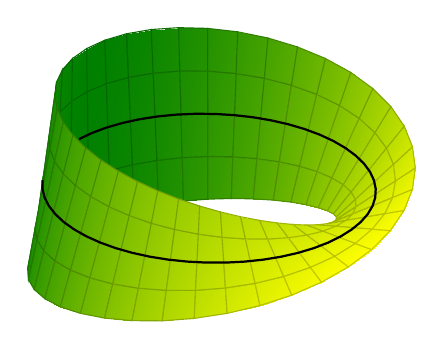
\begin{tikzpicture}
	  \begin{axis}[
	    hide axis,
	    view = {40}{40}
	  ]
	  \addplot3 [
	    surf,
	    colormap/greenyellow,
	    shader     = faceted interp,
	    point meta = x,
	    samples    = 40,
	    samples y  = 5,
	    z buffer   = sort,
	    domain     = 0:360,
	    y domain   =-0.5:0.5
	  ] (
	    {(1+0.5*y*cos(x/2)))*cos(x)},
	    {(1+0.5*y*cos(x/2)))*sin(x)},
	    {0.5*y*sin(x/2)}
	  );

	  \addplot3 [
	    samples=50,
	    domain=-145:180, % The domain needs to be adjusted manually,
			     % depending on the camera angle, unfortunately
	    samples y=0,
	    thick
	  ] (
	    {cos(x)},
	    {sin(x)},
	    {0}
	  );
	  \end{axis}
	\end{tikzpicture}
\end{center}

If a surface cannot be oriented, one cannot define the flux ``through'' that surface.

\subsection{Flux in Other Dimensions}

We've explored flux in three dimensions, but flux can be defined in any dimension
for a ``surface'' in that dimension, where ``surface'' means something for which a
consistent choice of normal vectors can be defined.  This means \emph{volumes} in four-dimensional
space  and curves in two-dimensional space can be considered surfaces.  In other dimensions,
one does not have the cross product, so an appeal to basic principles may be needed to compute
flux.

\begin{example}
	Let $\mathcal B$ be the boundary of $[0,1]\times[0,1]$
	oriented outward and let $\vec F(x,y)=(x^2,-y^2)$.  Compute the flux of $\vec F$
	through $\mathcal B$.

	XXX Finish
	
\end{example}


\subsection{Divergence}

Let $\vec F:\R^3\to\R^3$ be a vector field and suppose $\mathcal S$ is a 
sphere oriented outwards.  As we move $\mathcal S$ around,
the flux through $\mathcal S$ might change from positive to negative or negative to positive.
If we change the size of $\mathcal S$, again we might see a change in flux, and if
we changed both the size and the position of $\mathcal S$, we might be able to pinpoint
places in $\vec F$ where vectors are generally pointing away from each other (diverging)
and where they are generally pointing towards each other (converging).


The \emph{divergence}\index{divergence} of a vector field precisely measures
where a vector field is diverging or converging.  

\begin{definition}[Divergence]
	Let $\vec F:\R^3\to\R^3$ be a vector field and let $R_{\Delta x,\Delta y,\Delta z}(x,y,z)$
	be the surface of the box with lower left corner at $(x,y,z)$,
	side-lengths $\Delta x,\Delta y,\Delta z$,
	and oriented outwards\footnote{ Precisely, $R_{\Delta x,\Delta y,\Delta z}(x,y,z)$
	is the surface of  $[x,x+\Delta x]\times[y,y+\Delta y]\times[z,z+\Delta z]$ oriented outwards.}.
	The \emph{divergence} of $\vec F$ at the point $(x,y,z)$, notated as $\nabla \cdot \vec F(x,y,z)$
	is
	\[
		\nabla \cdot \vec F(x,y,z) = \lim_{\Delta x,\Delta y,\Delta z\to 0}
		\frac{\text{flux of }\vec F\text{ through }R_{\Delta x,\Delta y,\Delta z}(x,y,z)}
		{\text{area of }
		R_{\Delta x,\Delta y,\Delta z}(x,y,z)}.
	\]
\end{definition}

In plain language, the divergence of a vector field can be though of as the flux per unit volume
of that vector field.  Divergence in dimensions other than three is defined similarly.

\begin{example}
	Find the divergence of $\vec F(x,y,z)=(x,y,z)$ at the origin.

	XXX Finish
\end{example}

\begin{example}
	Estimate regions where the divergence is positive, negative, or zero
	for the following vector field plots.

	XXX Finish
\end{example}

The notation $\nabla \cdot \vec F$ comes from physics and is a handy pneumonic
for remembering quick way to compute divergence.  In order to see why this notation
makes sense, we need to work in some generality.

\bigskip
To keep the number of variables down, we will explore divergence in $\R^2$ for the moment.
Let $\vec F:\R^2\to\R^2$ a be a vector field defined by
$\vec F(x,y)=\mat{f_x(x,y)\\f_y(x,y)}$ and consider $R_{\Delta x,\Delta y}(x_0,y_0)$.
$R_{\Delta x,\Delta y}(x_0,y_0)$ has four sides, which we will label $L,R,T,B$.

XXX Figure

We will compute the approximate flux through these sides separately.  Consider 
$L=\{x_0\}\times[y_0,y_0+\Delta y]$ oriented to the left.  If $\Delta y$ is small,
$\vec F$ (along $L$) can be reasonably approximated by the constant vector
$\vec F(x_0,y_0)$  Therefore,
\[
	\Flux_{L}\vec F \approx \Delta y \mat{-1\\0}\cdot \vec F(x_0,y_0) = -\Delta y f_x(x_0,y_0).
\]
Similarly, near $R=\{x_0+\Delta x\}\times [y_0,y_0+\Delta y]$, $\vec F$ can be approximated
by $\vec F(x_0+\Delta x,y_0)$.  Since $R$ is oriented to the right, we have
\[
	\Flux_{R}\vec F \approx \Delta y \mat{1\\0}\cdot \vec F(x_0,y_0) = \Delta y f_x(x_0+\Delta x,y_0).
\]
Continuing the process, we compute
\[
	\Flux_{B}\vec F \approx -\Delta x\mat{0\\1}\cdot \vec F(x_0,y_0) = -\Delta x f_y(x_0,y_0),
\]
and
\[
	\Flux_{T}\vec F \approx \Delta x\mat{0\\1}\cdot \vec F(x_0,y_0+\Delta y) = \Delta x f_y(x_0,y_0+\Delta y).
\]
We're now ready to approximate the divergence of $\vec F$ at $(x_0,y_0)$.
\begin{align*}
	\nabla \cdot \vec F &\approx \frac{\Flux_R\vec F + \Flux_L\vec F + \Flux_T\vec F + \Flux_B\vec F}{\Delta x\Delta y}\\
		&= \frac{\Delta y\Big( f_x(x_0+\Delta x,y_0) - f_x(x_0,y_0)\Big)
		+\Delta x\Big( f_y(x_0,y_0+\Delta y) - f_y(x_0,y_0)\Big)}{\Delta x\Delta y}\\
		& = \frac{f_x(x_0+\Delta x,y_0) - f_x(x_0,y_0)}{\Delta x} + 
			\frac{f_y(x_0,y_0+\Delta y) - f_y(x_0,y_0)}{\Delta y},
\end{align*}
with equality following after we take a limit as $\Delta x,\Delta y\to 0$.  But some of these
limits look familiar!
\[
	\lim_{\Delta x\to 0} \frac{f_x(x_0+\Delta x,y_0) - f_x(x_0,y_0)}{\Delta x} 
	= \frac{\partial f_x}{\partial x}(x_0,y_0)
\]
and
\[
	\lim_{\Delta y\to 0} \frac{f_x(x_0,y_0+\Delta y) - f_x(x_0,y_0)}{\Delta y}
	= \frac{\partial f_y}{\partial y}(x_0,y_0).
\]
We conclude\footnote{ Of course, we had some sleight of hand in our derivation.  In order
to guarantee  all the limits involved exist and don't depend on particular choices
(like, why did we approximate $\vec F$ along $L$ by $\vec F(x_0,y_0)$ instead of
$\vec F(x_0,y_0+\tfrac{\Delta y}{2})$?) we need to assume that $\vec F$ is differentiable.
With that assumption, one can prove that the answer is the same regardless of choices
for first-order approximations.}
\[
	\nabla \cdot \vec F(x_0,y_0) = \frac{\partial f_x}{\partial x}(x_0,y_0)
	+ \frac{\partial f_y}{\partial y}(x_0,y_0).
\]

A very similar process shows that if $\vec G:\R^3\to\R^3$ with component functions
$g_x,g_y,g_z$, then
\[
	\nabla \cdot \vec G(x_0,y_0,z_0) = \frac{\partial g_x}{\partial x}(x_0,y_0,z_0)
	+ \frac{\partial g_y}{\partial y}(x_0,y_0, z_0) + \frac{\partial g_z}{\partial z}(x_0,y_0, z_0).
\]

In light of these formulas for divergence, the
pneumonic $\nabla \cdot \vec G$ makes some sense.  If we suspend our belief
that every mathematical sentence we write should have meaning, we can think of 
$\nabla =(\tfrac{\partial}{\partial x},\tfrac{\partial}{\partial y},\tfrac{\partial}{\partial z})$
and $\vec G=(g_x,g_y,g_z)$, then
\[
	\nabla \cdot \vec G=(\tfrac{\partial}{\partial x},\tfrac{\partial}{\partial y},\tfrac{\partial}{\partial z})
	\cdot 
	(g_x,g_y,g_z)
	=\tfrac{\partial g_x}{\partial x}+\tfrac{\partial g_y}{\partial y}+\tfrac{\partial g_z}{\partial z}
\]
is not bad as a memory aid\footnote{ There is a theory of operators where $\tfrac{\partial }{\partial w}$
has meaning by itself.  However, even in that framework, ``multiplication'' typically means 
scalar multiplication and not function application.  There's a bit of twisting one needs to do
to make something like $\nabla \cdot \vec G$ more than a pneumonic.}.  


\subsection{The Divergence Theorem}

Imagine a pond with various holes in its basin. Water flows in
from some of the holes and out from others.  If we consider $\vec V:\R^3\to\R^3$
to be the velocity of water in the pond, the divergence of $\vec V$ would
be positive at holes where water is flowing in and negative 
at holes where it is flowing out.  For this reason, we call points in a vector
field where the divergence is positive \emph{sources}\index{source}
and points where the divergence is negative \emph{sinks}\index{sink}.

If we enclose a region of the pond in a net and ask, ``what is the total
flux through the net\mbox{?}'' it is reasonable to expect that the flux
through the net is equal to the amount of water coming from sources minus
the amount coming from sinks.  The divergence theorem makes this reasoning
precise.

In order to properly state the divergence theorem, we need some notation.

\begin{definition}[Boundary]
	For a region $R\subseteq \R^n$, the \emph{boundary}\index{boundary}
	of $R$ is notated $\partial R$ and always comes with an outward orientation.
\end{definition}

Precisely defining what it means to be a boundary
of a region is tricky business.  Fortunately, your intuition will take you quite far.
For example, the boundary of a disk is a circle, the boundary of a filled in cube
is the surface of that cube and the boundary of an interval consists of its endpoints.

XXX Figure

It's important to note that boundaries can be empty.  For example, the boundary
of a single point is empty.  The boundary of a circle is also empty (it has no ``ends'').
In fact, for any nice region $R$, it holds that $\partial (\partial R) = \emptyset$.


We can now precisely state the \emph{divergence theorem}\index{divergence theorem}
(also known as \emph{Gauss's theorem}\index{Gauss's theorem} or 
\emph{Ostrogradsky's theorem}\index{Ostrogradsky's theorem}).

\begin{theorem}[Divergence Theorem]
	Let $\vec F$ be a vector field and $R$ be a region.  Then
	\[
		\Flux_{\partial R} \vec F = \int_{R} \nabla \cdot \vec F.
	\]
\end{theorem}

The divergence theorem holds in all dimensions, but it is sometimes
stated in $\R^3$ strictly in terms of integrals as
\[
	\iint_{\partial R} \vec F\cdot \hat n \d V_{\partial R}
	=\iiint_R \nabla \cdot \vec F \d V_{R}
\]
where $\hat n$ is a unit normal vector to $\partial R$, and $\d V_{\partial R}$
and $\d V_R$ are the volume forms for $\partial R$ and $R$, respectively.

\begin{example}
	Verify the divergence theorem for the vector field $\vec F$=...
	on the region $R=...$

	XXX Finish
\end{example}

\bigskip
In words, the divergence theorem states that the flux through a
boundary equals the sum of the divergence (sources and sinks)
on its interior, and, though proving the divergence theorem can be challenging,
the essential idea is simple and beautiful.

Let $\vec F$ be a vector field, and 
consider two adjacent squares, $A$ and $B$, both oriented outwards.

XXX Figure

Let $R=A\cup B$ be the rectangular region formed by joining $A$ and $B$.  Now,
\[
	\Flux_R \vec F = \Flux_A\vec F+\Flux_B \vec F
\]
because the contributions to flux on the common edge shared by $A$ and $B$
are opposite and cancel.  Now consider a more complicated region $X$.  If
we chop $X$ into tiny squares each called $\Delta X$, we see that
\[
	\Flux_{\partial X} \vec F = \sum_{\partial \Delta X} \Flux_{\partial \Delta X} \vec F,
\]
because, again, flux through any interior edges cancels out.  But, this means
the only flux that actually contributes is the flux along the boundary.

XXX Figure

Of course, we were considering $\Flux_{\partial X}\vec F$ to begin with,
so only the boundary should matter.  However, as the area of $\Delta X$ gets very tiny,
\[
	\Flux_{\partial \Delta X} \vec F \approx (\text{area of }\Delta X)(\nabla \cdot \vec F
	\text{ at }\Delta X).
\]
After taking a limit, we get the divergence theorem.


\section{Circulation and Curl}

Given a vector field and a surface, it is natural
to ask what the flux of the vector field through the surface is.
Given a vector field and a closed curve\index{closed curve} (a curve that loops back
to itself), it is natural to ask what the \emph{circulation}\index{circulation}
of the vector field through the curve is.  That is, given a loop $L$,
how much would a vector field ``push'' something around $L$.

Circulation is closely related to the concept of work, except that
it only applies to closed curves.

\begin{definition}[Circulation]
	Given an oriented, closed $C$ and a vector field $\vec F$, the 
	\emph{circulation} of $\vec F$ around $C$ is the amount
	of work done by $\vec F$ while traversing $C$.  As a
	vector line integral,
	\[
		\Circ_C\vec F = \int_C \vec F \cdot \d \vec r.
	\]
\end{definition}

To visualize the circulation of $\vec F$ around a curve $C$, imagine that
$C$ is a roller coaster track, weightless in space.  You then place a car on
this track and let it get pushed by $\vec F$.  If it makes a complete loop and
continues in the same direction that $C$ is oriented, $\Circ_C\vec F$ is positive.
If it makes a loop and continues in the opposite direction to how $C$ is 
oriented, $\Circ_C \vec F$ is negative.

\begin{example}
	Find the circulation of ...

	XXX Finish
\end{example}

Just like the divergence of a vector field is the amount of flux per unit area,
we have an idea of ``circulation per unit area,'' which is called \emph{curl}\index{curl}.
However, there is a problem.
At a point, there is fundamentally only \emph{one} tiny volume centered at that
point\footnote{ When we defined divergence, we used a cube, but we could have used
a sphere.}, however, at a point, there are \emph{infinitely} many tiny curves 
circulating that point---at a point $\vec p$,
for every choice of vector $\vec n$, we could consider a tiny curve going around 
$\vec p$ and contained in the plane with normal vector $\vec n$.  
Thus, curl cannot be represented by a single scalar quantity.


\begin{definition}[Curl]
	For a unit vector $\vec v$, 
	let $R^{\vec v}_{\Delta a,\Delta b}(x,y,z)$ be the perimeter
	of a rectangle with lower left
	corner at $(x,y,z)$, side lengths $\Delta a$ and $\Delta b$, contained
	in a plane with normal vector $\vec v$, and oriented counter-clockwise.

	Let $\vec F:\R^3\to\R^3$ be a vector field.  The \emph{$\vec v$
	component of the curl of $\vec F$ at the point $(x,y,z)$} is
	\[
		\Curl_{\vec v}\vec F(x,y,z) = \lim_{\Delta a,\Delta b\to 0}
		\frac{
			\text{circulation of }\vec F\text{ around }R^{\vec v}_{\Delta a,\Delta b}(x,y,z)
			}{
			\text{area of }R^{\vec v}_{\Delta a,\Delta b}(x,y,z)}.
	\]

	The \emph{curl} of $\vec F$ at the point $(x,y,z)$, notated
	$\nabla \times \vec F(x,y,z)$, is the vector so that
	\[\Big(\nabla \times \vec F(x,y,z)\Big)\cdot \vec v = \Curl_{\vec v}\vec F(x,y,z).\]
\end{definition}

It's important to notice that for a vector field $\vec F$
and a unit vector $\vec v$, the \emph{component} of the curl of $\vec F$ in the direction
$\vec v$ is a scalar, but \emph{the} curl  of $\vec F$ is encapsulated as a vector.

A priori, $\nabla \times \vec F$ might be hard to compute, but its definition 
makes it workable.  If we assume $\nabla \times \vec F(x,y,z)=(a,b,c)$, then
\begin{align*}
	a &= \nabla \times \vec F(x,y,z)\cdot \xhat = \Curl_{\xhat} \vec F(x,y,z)\\
	b &= \nabla \times \vec F(x,y,z)\cdot \yhat = \Curl_{\yhat} \vec F(x,y,z)\\
	c &= \nabla \times \vec F(x,y,z)\cdot \zhat = \Curl_{\zhat} \vec F(x,y,z),
\end{align*}
and $R^{\xhat}_{\Delta a,\Delta b}(x,y,z)$, $R^{\yhat}_{\Delta a,\Delta b}(x,y,z)$,
and
$R^{\zhat}_{\Delta a,\Delta b}(x,y,z)$ are workable rectangles\footnote{ Pun intended.}.

\begin{example}
	XXX Finish
\end{example}

Again, like divergence, the $\nabla \times \vec F$ notation serves as a pneumonic
for computing curl.  The derivation of a formula for the components of curl
is very similar to the derivation for the components of divergence, so we won't go
through it here.  When all is said and done, if $\vec F(x,y,z) = \Big(f_x(x,y,z),f_y(x,y,z),
f_z(x,y,z)\Big)$, then
\[
	\nabla \times \vec F = \mat{
		\tfrac{\partial f_z}{\partial y} - \tfrac{\partial f_y}{\partial z}\\[4pt]
		\tfrac{\partial f_x}{\partial z} - \tfrac{\partial f_z}{\partial x}\\[4pt]
		\tfrac{\partial f_y}{\partial x} - \tfrac{\partial f_x}{\partial y}
		}.
\]

\subsection{Closed Vector Fields}
We already have the tools to deduce some theorems about curl and circulation.
In particular, if $\vec F=\nabla f$ is a conservative vector field, then the circulation
around any closed loop should be zero.  Therefore, every component of the curl of
$\vec F$ is zero.

\begin{theorem}
	If $\vec F=\nabla f$ is a conservative vector field, then $\nabla \times \vec F=\vec 0$.
\end{theorem}

The converse of this statement isn't necessarily true.

\begin{definition}[Closed Vector Field]
	A vector field $\vec F:\R^3\to\R^3$ is called \emph{closed}\index{closed}
	if $\nabla \times \vec F=\vec 0$.
\end{definition}

If we write out in components what it means for a vector field to be closed,
we see that $\vec F$ is closed exactly when it passes the \emph{screening test}
from Section \ref{SECSCREENING}.  We already know that passing the screening test
is necessary but not sufficient for showing a vector field is conservative.

\begin{example}
	Show that ... is closed by not conservative

	XXX Finish
\end{example}

However, there are times when closed does imply conservative.  In particular,
if a region could be deformed to a ball, a vector field
being closed on that region implies that it's conservative.

\begin{theorem}[Poincar\'e Lemma]
	Let $R$ be a region that can be deformed into
	a ball.  Then, for a vector field $\vec F$,
	if $\nabla\times \vec F=\vec 0$ on the region $R$,
	it must be that $\vec F$ is conservative.
\end{theorem}

\begin{example}
	XXX show that the region from the previous example cannot
	be deformed into a ball.
\end{example}
xx

\subsection{Curl in Other Dimensions}

The concept of circulation is defined for vector fields of any dimension.
Therefore, we can define the analog of curl in any dimension.  However,
in other dimensions, curl looks a little different than in three dimensions.

For example, if $\vec F:\R^\to\R^2$, then the curl of $\vec F$ takes the form
of a scalar.  Why?  Well, if we specify the normal vector of a plane in
$\R^2$, there aren't that many choices.  We can either specify the normal 
vector to be ``up,'' giving the plane a counter-clockwise orientation, or
we can specify it to be ``down,'' giving it a clockwise orientation.  Therefore,
there is only one \emph{component} to the curl of a vector field in $\R^2$.

\begin{example}
	XXX Example of curl of vector field in $\R^2$
\end{example}

If, $G:\R^4\to\R^4$, things are even stranger.  To specify the orientation
of a plane in $\R^4$, you need a \emph{bi-vector}\index{bi-vector}.  After 
some fiddling, you can conclude that to represent the curl of $\vec G$, you
need \emph{six} components\footnote{ Surprise, it's not eight!}.

In general, to represent curl in $\R^n$, you need a $n(n-1)/2$ components.
Of course, there are better ways to talk about curl in $\R^n$ than vectors
(for example, differential forms\index{differential forms}).

\subsection{Stokes's Theorem}

It may have struck you that circulation through adjacent regions cancels
in a similar way to how flux canceled.

Let $A$ and $B$ be the perimeter of two adjacent squares oriented counter-clockwise,
and let $R$ be the perimeter of the rectangle containing $A$ and $B$ oriented 
counter-clockwise.

XXX Figure

We see that because the shared edge between $A$ and $B$ is oriented in opposite
directions, the contribution to circulation along that edge cancels.  Thus, for a vector
field $\vec F$,
\[
	\Circ_R\vec F = \Circ_A\vec F+\Circ_B \vec F. 
\]

We will 
now play a nearly-identical trick as in the derivation of the divergence theorem.  However,
we need to sort out the issue of \emph{orientation} again.

For a volume $V$ in $\R^3$ or an area $A$ in $\R^2$, the orientation
of $\partial V$ and $\partial A$ is ``outward.''  However, what if we have
a surface $S$ in $\R^3$.  If $S$ is a surface, then $\partial S$ is
a curve, and there is no ``outward'' for a curve in $\R^3$.  There is
however a forward and a backwards.  We will define the orientation
of $\partial S$ according to the right-hand rule.

Without getting overly technical, we say that \emph{$\partial S$ is oriented
consistently with $S$ according to the right hand rule} if the following condition
holds.  Let $s\in\partial S$ and let $\vec t$ be the tangent vector to $\partial S$
aligned with $\partial S$'s orientation; let $\vec n$ be a normal vector to $S$ aligned
with its orientation; then, $\vec t\times \vec n$ points ``away'' from the boundary.

XXX Figure


Now we are ready explore the analog of the divergence theorem, Stokes's theorem\index{Stokes's 
theorem}.
Consider a region $X$.  If
we chop $X$ into tiny squares each called $\Delta X$, we see that
\[
	\Circ_{\partial X} \vec F = \sum_{\partial \Delta X} \Circ_{\partial \Delta X} \vec F,
\]
because circulation along any interior edges cancels out.

XXX Figure

However, as the area of $\Delta X$ gets very tiny,
\[
	\Circ_{\partial \Delta X} \vec F \approx (\text{area of }\Delta X)(\nabla \times \vec F
	\text{ at }\Delta X)\cdot \vec n,
\]
where $\vec n$ is a unit normal vector to $\Delta X$.  But, 
\[ 
	(\text{area of }\Delta X)(\nabla \times \vec F
	\text{ at }\Delta X)\cdot \vec n = \Flux_{\Delta X}(\nabla \times \vec F\text{ at }\Delta X).
\]
After taking a limit, the approximation becomes exact and we get Stokes's theorem
relating flux, circulation, and curl.

\begin{theorem}[Stokes's Theorem]
	Let $S\subset \R^3$ be an oriented surface and let $\vec F:\R^3\to\R^3$.  Then,
	\[
		\Circ_{\partial R} \vec F = \Flux_{R}(\nabla \times \vec F).
	\]
\end{theorem}

We can rephrase Stokes's theorem in terms of integrals.  That is, for an oriented
surface $S$ and vector field $\vec F:\R^3\to\R^3$,
\[
	\int_{\partial S} \vec F\cdot \d\vec r = \iint_S (\nabla \times \vec F)\cdot
	\hat n\d V_S,
\]
where $\hat n$ is the unit normal vector to $S$ with appropriate orientation and 
$\d V_S$ is the volume form for $S$.  Phrased this way, there is a striking similarity
between Stokes's theorem and the divergence theorem.

\begin{example}
	Use Stoke's theorem to calculate ...

	XXX Finish
\end{example}



